\documentclass[11pt]{article}

\usepackage{amsmath}
\usepackage{float}
\usepackage{graphicx}

\author{Maximilian Mayerl, Alexander Schl\"ogl, Benedikt Wimmer}
\title{Assignment 2, Report}

\begin{document}
    \maketitle

    \section{Implementation}
    \label{sec:implementation}
    The implementation was carried out in four steps, as suggested by the exercise sheet.


        \subsection{Computing Partial Derivatives}
        \label{sec:partderiv}
        The first step was to compute the partial derivatives of the linear basis functions. This was implemented in \texttt{LinTriElement::ComputeBasisDeriv}. Our approach works as follows:

        \begin{enumerate}
            \item Get the three vectors (x$_1$, y$_1$), (x$_2$, y$_2$) and (x$_3$, y$_3$) from the \texttt{FEModel} via its \texttt{GetNodePosition} method.
            \item Put the three vectors into a \texttt{Matrix3x3} in order to solve the corresponding linear equation.
            \item Solve the linear system by inverting the matrix via the \texttt{Matrix3x3::Inverse} method.
        \end{enumerate}

        The partial derivatives were then simply recovered from the inverted matrix.         
        
        
        \subsection{Assembling Global Stiffness Matrix}
        \label{sec:stiffmat}
        The next step was to assemble the global stiffness matrix. This was implemented in \texttt{LinTriElement::AssembleElement}. 

        For this, we first calculate the derivatives of the basis functions by calling the method implemented in \ref{sec:partderiv}. After that, we iterate over the elements of the vector of partial derivatives with two nested loops to get every combination of the derivatives. An individual contribution is then calculated as shown in the exercise sheet.


        \subsection{Determining Right-Hand Side Vector}
        \label{sec:rhsvector}
        The third step was to determine the right-hand side vector of the \texttt{FEModel}. This was implemented in \texttt{FEModel::ComputeRHS}. Our solution for this task works as follows:

        \begin{enumerate}
            \item Clear the right-hand side vector by filling it with zeros.
            \item For every node, check for every triangle if it contains that node.
            \item If yes, add $A_e \cdot f(x_c, y_c) \cdot N_j(x_c, y_c)$.
        \end{enumerate}       


        \subsection{Calculate Error}
        \label{sec:solveerror}
        The last step was to determine the accuracy of our implementation. This was implemented in \texttt{FEModel::ComputeError}. For this, we first determine the absolute error vector between the numerical solution and the analytical solution. After that, we calculate the inner product error norm based on this absolute error vector.


    \section{Results}
    \label{sec:results}
    The visualization produced by the provided framework for our solution looks as shown in Figure \ref{fig:res}.

    \begin{figure}[H]
        \centering
        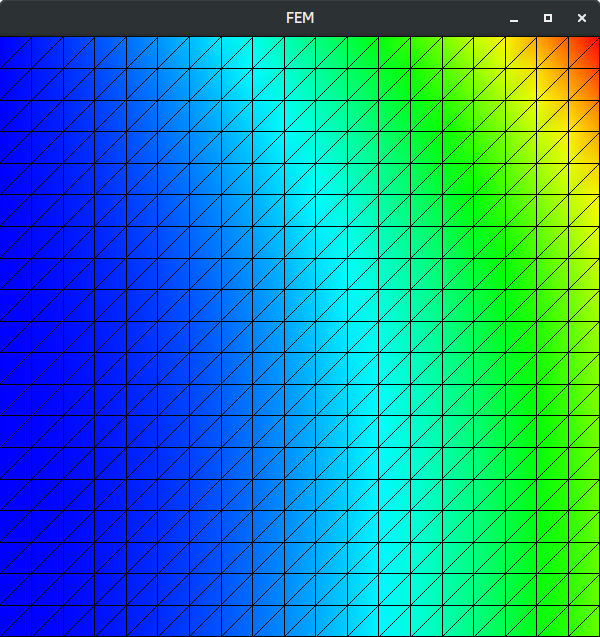
\includegraphics[width=0.5\textwidth]{res}
        \caption{Visualization of our result.}
        \label{fig:res}
    \end{figure}


    The visualization produced by the provided framework for the error of our solution looks as shown in Figure \ref{fig:error}.

    \begin{figure}[H]
        \centering
        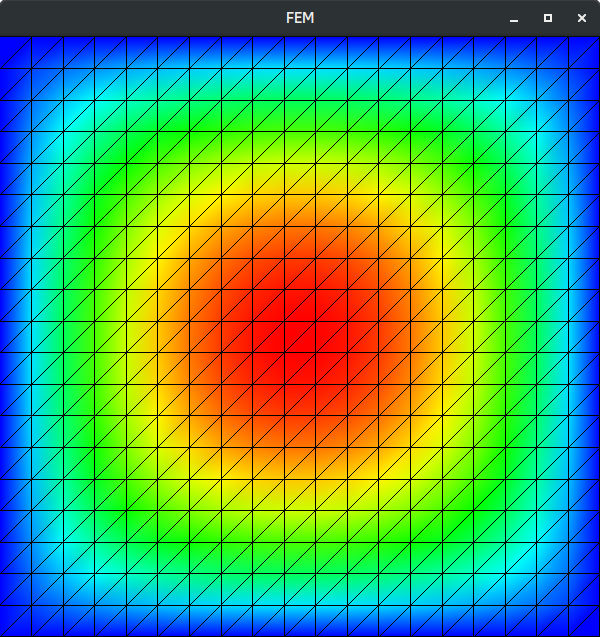
\includegraphics[width=0.5\textwidth]{error}
        \caption{Visualization of our error.}
        \label{fig:error}
    \end{figure}

    The error norm was calculated as $3.55799 \cdot 10^{-10}$.


\end{document}
